%% Dokumentklasse KOMA-Script Report
\documentclass[paper=a4, 12pt]{scrreprt}
%% Encoding UTF8
\usepackage[utf8]{inputenc}
%%Use Source Sans Pro Textstyle
\usepackage[default]{sourcesanspro}
%% 8 Bit Aufloesung der Buchstaben
\usepackage[T1]{fontenc}
%% Seitenraender
%\usepackage[scale=0.72]{geometry}
\usepackage[scale=0.72, twoside, bindingoffset=2mm]{geometry}

\usepackage[onehalfspacing]{setspace}

%% Spracheinstellungen
% \usepackage[english, naustrian]{babel} % your native language must be the last one!!
\usepackage[german]{babel} % your native language must be the last one!!
%% erweiterte Farbenpalette
\usepackage[dvipsnames]{xcolor}
%% Abbildungen
\usepackage{graphicx}
%%Tabelen mit Farbe (cellcolor)
\usepackage{tabulary}
\usepackage{colortbl}
\PassOptionsToPackage{dvipsnames,svgnames,table}{xcolor}
%% Tabellen (erweitert)
\usepackage{tabularx}
%% TikZ + Circuit-TikZ (fuer Schaltungen)
\usepackage[europeanresistors, europeaninductors]{circuitikz}
%% Nuetzliche TikZ Libraries
\usetikzlibrary{arrows, automata, positioning}
%% mathematik
\usepackage{amsmath, amssymb}
%%Formelbeschreibung
\newenvironment{conditions}
  {\par\vspace{\abovedisplayskip}\noindent\begin{tabular}{>{$}l<{$} @{${}...{}$} l}}
  {\end{tabular}\par\vspace{\belowdisplayskip}}
%\usepackage{mathtools}	
%% pdf-einbindung
\usepackage{pdfpages}
%% scource-code einbindung
\usepackage{listings, scrhack} %scrhack vermeidet Umschaltung auf KOMA
% Floats..
\usepackage{courier}
%% euro-symbol
\usepackage{eurosym}
%% landcsape-seiten ermöglichen
\usepackage{lscape}

%% Diplomarbeits-Format
\usepackage{srdpdipa}

%% Abkuerzungsverzeichnis
\usepackage[]{acronym}

%% Todos
\setlength{\marginparwidth}{2cm}
\usepackage[]{todonotes}

%% Ganttdiagramme
\usepackage{pgfgantt}

%% Subfigures
\usepackage[lofdepth]{subfig}

%% Für Quellenangaben unter Bildern
\newcommand*{\quelle}[1]{\par\raggedleft\footnotesize Quelle:~#1}

%% Listings (Code)
\usepackage{listings}
\usepackage{color}


%% CUSTOM PACKAGES

% \usepackage{chngcntr}
% \counterwithin{figure}{subsection}
% \counterwithin{table}{subsection}

\usepackage{multirow}

\definecolor{dkgreen}{rgb}{0,0.6,0}
\definecolor{gray}{rgb}{0.5,0.5,0.5}
\definecolor{mauve}{rgb}{0.58,0,0.82}

\lstset{frame=none,
  language=Python,
  aboveskip=3mm,
  belowskip=3mm,
  showstringspaces=false,
  columns=flexible,
  basicstyle={\small\ttfamily},
  numbers=left,
  numberstyle=\tiny\color{gray},
  keywordstyle=\color{blue},
  commentstyle=\color{dkgreen},
  stringstyle=\color{mauve},
  breaklines=true,
  breakatwhitespace=true,
  tabsize=3
}

\lstset{literate=%
  {Ö}{{\"O}}1
  {Ä}{{\"A}}1
  {Ü}{{\"U}}1
  {ß}{{\ss}}1
  {ü}{{\"u}}1
  {ä}{{\"a}}1
  {ö}{{\"o}}1
}

%% TIKZ Flowcharts
\usepackage{tikz}
\usetikzlibrary{shapes.geometric, arrows}

\tikzstyle{startstop} = [rectangle, rounded corners, minimum width=3cm, minimum height=1cm,text centered, draw=black, fill=green!32]
\tikzstyle{io} = [trapezium, trapezium left angle=70, trapezium right angle=110, minimum width=3cm, minimum height=1cm, text centered, draw=black, fill=red!35]
\tikzstyle{process} = [rectangle, minimum width=3cm, minimum height=1cm, text centered, draw=black, fill=cyan!32]
\tikzstyle{decision} = [diamond, minimum width=3cm, minimum height=1cm, text centered, draw=black, fill=orange!42]

\tikzstyle{arrow} = [thick,->,>=stealth]

% Leere Seite mit Kopf- und Fußzeile
\def\blankpage{
	\clearpage
	\null
	\clearpage
}

% Leere Seite ohne Kopf- und Fußzeile 
\def\blankemptypage{
	\clearpage
	\thispagestyle{empty}
	\null
	\clearpage
}

%% definitsionen =====================================%%
\dataSchool{HTBLuVA St. Pölten}
\dataDepartment{Höhere Lehranstalt für Elektronik und Technische Informatik}
\dataSubdepartment{Ausbildungsschwerpunkte Wireless Systems/Embedded Systems}
\dataSession{2023/24}


\title{Battery Management System}
\author{Kaiser Thomas \and Tucek Markus}
\date{\today}
\place{St. P\"olten}
\professor{\and}



%%====================================================%%

% Hyperlinks im Dokument
\usepackage[colorlinks=true,
    linkcolor=black,
    citecolor=black,
    bookmarks=true,
    urlcolor=black,
    bookmarksopen=true]{hyperref}

\begin{document}

\frontmatter

%% titelseite ==========================================%%
\maketitle
%%======================================================%%

%% komplett leere seite ================================%%
\newpage\null\thispagestyle{empty}%\newpage
%%======================================================%%

%% eidesstattliche erklärung ===========================%%
\begin{affidavit}
    \unterschrift{Kaiser Thomas}
    \unterschrift{Tucek Markus}
\end{affidavit}
%%======================================================%%
\blankemptypage
%% dokumentation (deutsch/englisch) ====================%%
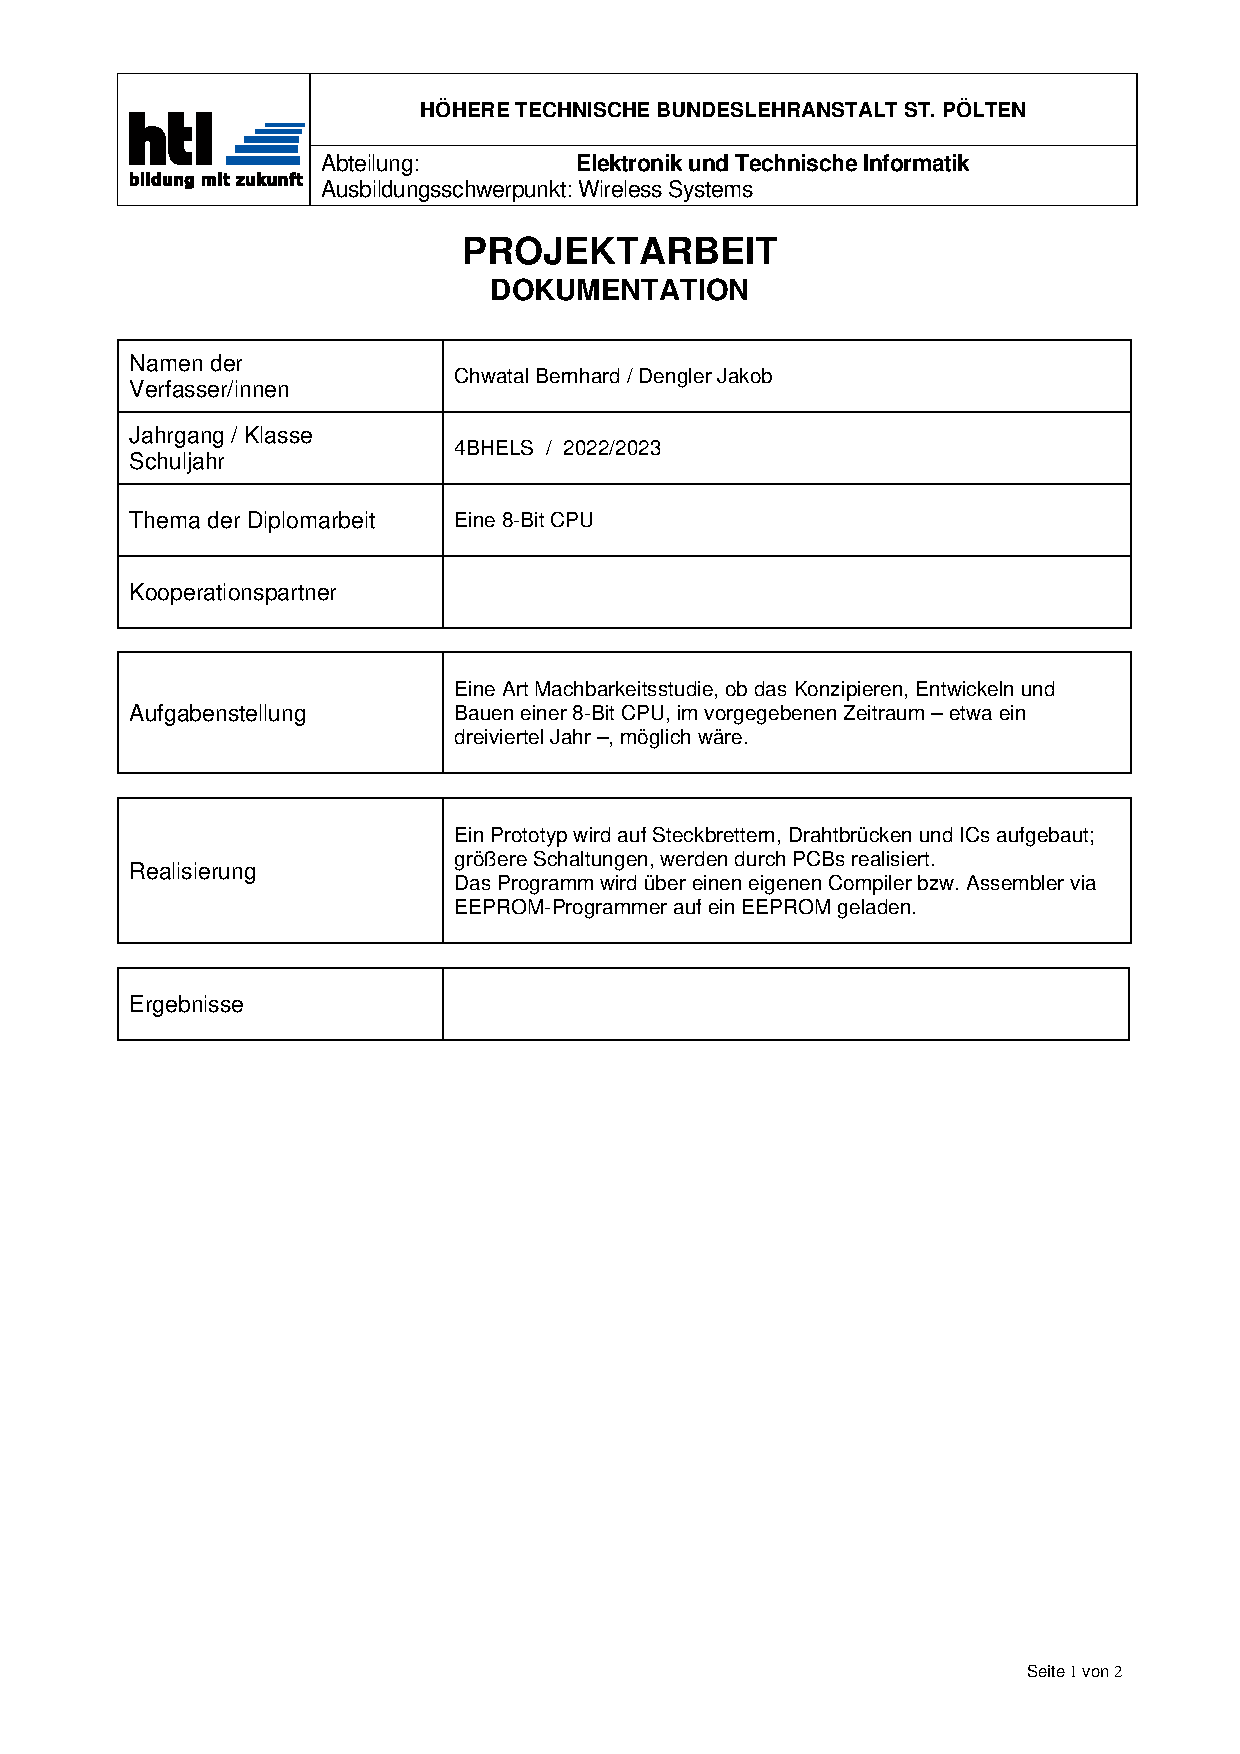
\includepdf[pages=1-2]{pdfs/DiplArbeit_DE.pdf}                 %Dokumentation(PDF) einfügen
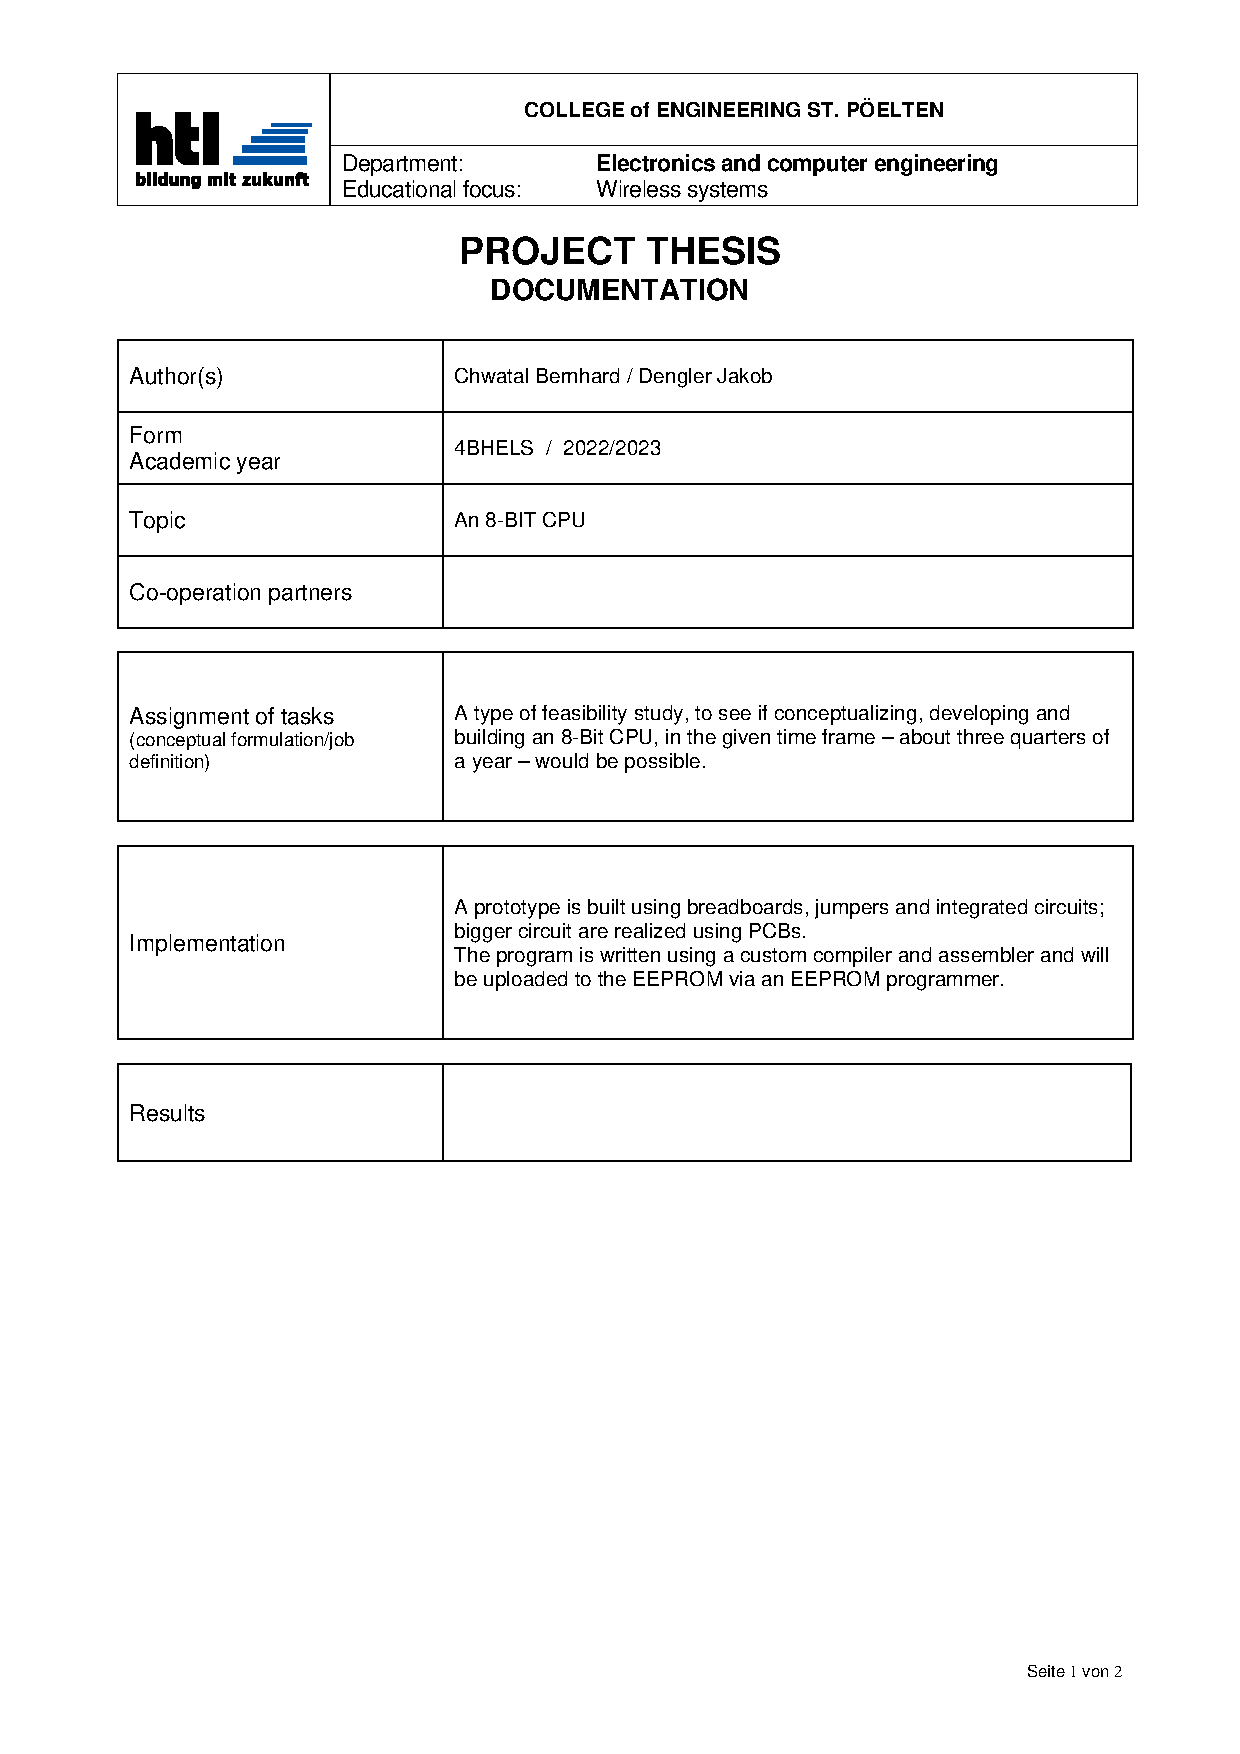
\includepdf[pages=1-2]{pdfs/DiplArbeit_EN.pdf}                 %Dokumentation(PDF) einfügen
%%======================================================%%

%% inhaltsverzeichnis ==================================%%
\renewcommand*\chapterpagestyle{scrheadings}
\tableofcontents
\responsible{Kaiser Thomas, Tucek Markus}
%%======================================================%%

%% HAUPTTEIL ===========================================%%

\mainmatter

% --- Einleitung ---
\chapter{Einleitung}

\responsible{Thomas Kaiser, Markus Tucek}

\section{Ausgangslage}

\section{Zielsetzung}

\subsection{Individuelle Zielsetzung Thomas Kaiser}

\subsection{Individuelle Zielsetzung Markus Tucek}

% --- Master ---
\chapter{Master}

\responsible{Thomas Kaiser}

\section{Anforderungsanalyse}

\subsection{Galvanische Trennung}

\subsection{Zündungserkennung}

\subsection{CAN-Controller}

\subsection{RS485}

\subsection{WLAN-Controller}

\subsection{Klemmverbindungen}

\subsection{externer Status}



%% Abbildungsverzeichnis %===============================%%    + Evnt Tabellenverzeichnis + Abkürzungen
\setcounter{lofdepth}{2}
\dipalistoffigures

%% Tabellenverzeichnis %===============================%%
\setcounter{lotdepth}{2}
\dipalistoftables

%% Danksagung
%================================%%
% \include{files/danksagungen}                                    %Danksagung(LaTeX File) einfügen



%%Zeitnachweise
%===============================%%
%
%\include{files/zeitnachweise}                                   %Zeitnachweise(LaTeX File) einfügen

%%USB Verzeichnis
%\include{files/USBVerzeichnis.tex}

%%Betreuungsprotokolle
%==========================================
%
%\chapter{Betreuungsprotokolle}
%%\includepdf[pages=-]{pdfs/besprechungsprotokoll_1.pdf}          %Besprechunsprotokoll(PDF) einfügen
%%\includepdf[pages=-]{pdfs/besprechungsprotokoll_2.pdf}
%%\includepdf[pages=-]{pdfs/besprechungsprotokoll_3.pdf}
%%usw....

\end{document}